
\section{Loss functions and performance metrics}

\newcommand{\autoplots}[1]{
    \begin{tikzpicture}
        \begin{axis}[
            height=5.3cm,
            width=9cm,
            xlabel={Horsepower},
            ylabel={Miles per gallon},
            xmin=41,
            xmax=236,
            ymin=6,
            ymax=49.6,
            xtick pos=bottom,
            ytick pos=left
        ]

            \ifnum#1<3
                \addplot[
                    only marks,
                    mark=*,
                    color=blue,
                    opacity=0.1
                ] table[
                    col sep=comma,
                    y=mpg,
                    x=horsepower
                ] {data/Auto.csv};
            \fi
            \ifnum#1=3
                \addplot[
                    only marks,
                    mark=*,
                    color=blue,
                    opacity=0.02
                ] table[
                    col sep=comma,
                    y=mpg,
                    x=horsepower
                ] {data/Auto.csv};
                \addplot[
                    only marks,
                    mark=*,
                    color=blue,
                    opacity=0.5
                ] coordinates {
                    (72, 22)
                    (100, 19)
                    (137, 14)
                    (198, 15)
                };
                \draw[densely dotted, thick]
                    (axis cs: 72, 22) --
                    (axis cs: 72, 39.936 - 72*0.158) --
                    (axis cs: 72 - 16, 39.936 - 72*0.158) --
                    (axis cs: 72 - 16, 22) -- cycle;
                \draw[densely dotted, thick]
                    (axis cs: 100, 19) --
                    (axis cs: 100, 39.936 - 100*0.158) --
                    (axis cs: 100 - 12, 39.936 - 100*0.158) --
                    (axis cs: 100 - 12, 19) -- cycle;
                \draw[densely dotted, thick]
                    (axis cs: 137, 14) --
                    (axis cs: 137, 39.936 - 137*0.158) --
                    (axis cs: 137 - 10, 39.936 - 137*0.158) --
                    (axis cs: 137 - 10, 14) -- cycle;
                \draw[densely dotted, thick]
                    (axis cs: 198, 15) --
                    (axis cs: 198, 39.936 - 198*0.158) --
                    (axis cs: 198 + 14, 39.936 - 198*0.158) --
                    (axis cs: 198 + 14, 15) -- cycle;
            \fi
            \ifnum#1>3
                \addplot[
                    only marks,
                    mark=*,
                    color=blue,
                    opacity=0.1
                ] table[
                    col sep=comma,
                    y=mpg,
                    x=horsepower
                ] {data/Auto.csv};
            \fi


            \ifnum#1>1
                \addplot[
                    domain=41:236,
                    very thick,
                    red
                ] {39.935861 - 0.157845 * x};
                \node[anchor=north east,font=\small\selectfont,red] at (axis cs: 230, 46.6) {
                    $\hat{y}=39.936 - 0.158x$
                };
            \fi

            \ifnum#1>3
                \addplot[
                    domain=41:236,
                    very thick,
                    teal
                ] {40.419 - 0.165 * x};
                \node[anchor=north east,font=\small\selectfont,teal] at (axis cs: 230, 42) {
                    $\hat{y}=40.419 - 0.165x$
                };
            \fi
        \end{axis}
    \end{tikzpicture}
}

\newsavebox{\autodata}
\sbox{\autodata}{\autoplots{1}}
\newsavebox{\automsemodel}
\sbox{\automsemodel}{\autoplots{2}}
\newsavebox{\automseloss}
\sbox{\automseloss}{\autoplots{3}}
\newsavebox{\automsemae}
\sbox{\automsemae}{\autoplots{4}}

\newcommand{\tabplot}[1]{
    \ifnum#1<5
        \def\ylabel{Tolerance-based accuracy}
    \fi
    \ifnum#1=5
        \def\ylabel{Mean squared error}
    \fi
    \ifnum#1=1
        \def\xlabel{$\hat{y}$}
        \def\xmin{19.5}
        \def\xmax{24.5}
        \def\xticks{{20, 21, 22, 23, 24}}
        \def\xticklabels{20, 21, 22, 23, 24}
    \fi
    \ifnum#1>1
        \def\xlabel{$\beta_1$}
        \def\xmin{19.5}
        \def\xmax{24.5}
        \def\xticks{{20, 21, 22, 23, 24}}
    \fi
    \ifnum#1=2
        \def\xticklabels{?,?,?,?,?}
    \fi
    \ifnum#1>2
        \def\xticklabels{0.277, 0.291, 0.305, 0.319, 0.333}
    \fi
    \begin{tikzpicture}
        \begin{axis}[
            height=4.5cm,
            width=8cm,
            ylabel=\footnotesize{\ylabel},
            ymin=-0.1,
            ymax=1.1,
            ytick={0, 1},
            xlabel=\footnotesize{\xlabel},
            xmin=\xmin,
            xmax=\xmax,
            xtick={\xticks},
            xtick pos=bottom,
            ytick pos=left,
            xticklabels/.expanded={\xticklabels}
        ]

            \ifnum#1<5
                \addplot[red, thick] coordinates {
                    (19, 1)
                    (21, 1)
                    (21, 0)
                    (23, 0)
                    (23, 1)
                    (25, 1)
                };
            \fi

            \ifnum#1=4
                \node[fill=red, inner sep=3pt, circle] at (axis cs: 23.6, 1) {};
            \fi

            \ifnum#1=5
                \addplot[
                    red,
                    thick,
                    domain=19:25,
                    samples=100
                ] {(x-22)^2/5};
                \node[fill=red, inner sep=3pt, circle] at (axis cs: 23.6, 1.6^2/5) {};
                \draw[-stealth, very thick] (axis cs: 23.527, 1.527^2/5) -- (axis cs: 23.3, 1.3^2/5 - 0);
            \fi
        \end{axis}
    \end{tikzpicture}
}

\newsavebox{\lossvsprediction}
\sbox{\lossvsprediction}{\tabplot{1}}
\newsavebox{\lossvsbeta}
\sbox{\lossvsbeta}{\tabplot{2}}
\newsavebox{\lossvsknownbeta}
\sbox{\lossvsknownbeta}{\tabplot{3}}
\newsavebox{\losspoint}
\sbox{\losspoint}{\tabplot{4}}
\newsavebox{\lossmse}
\sbox{\lossmse}{\tabplot{5}}

\begin{frame}{Loss functions and performance metrics}
    \only<1>{
        \begin{center}
        \textbf{Loss functions versus performance metrics}\\
        \end{center}
        \underline{Commonalities}\\[-0.1cm]
        \begin{itemize}
            \item Allows us to evaluate the performance of a model
            \item Typically on the form $f(y, \hat{y})$
        \end{itemize}
        \vspace{-0.2cm}\underline{Loss functions}\\[-0.1cm]
        \begin{itemize}
            \item Tailored specifically for mathematical optimization of models
        \end{itemize}
        \vspace{-0.2cm}\underline{Performance metrics}\\[-0.1cm]
        \begin{itemize}
            \item Tailored specifically for interpretation of model performance by humans
        \end{itemize}
    }
    \only<2-17>{
        \begin{tikzpicture}
            \node[] at (-5.25, -3.5) {};
            \node[] at (5.25, 3.5) {};

            \visible<2-6>{
                \node[] at (0, -2.1) {
                    $\text{mse} (y, \hat{y})= \dfrac{1}{n}\sum\limits_{i=0}^{n} (y_i - \hat{y}_i)^2$
                };
            }
            \visible<3,6>{
                \node[] at (-0.6, 1) {
                    \usebox{\automsemodel}
                };
            }
            \visible<4-5>{
                \node[] at (-0.6, 1) {
                    \usebox{\automseloss}
                };
            }
            \visible<5>{
                \node[] at (0.125, -3.1) {
                    $=23.94$
                };
            }
            \visible<6>{
                \node[] at (-0.07, -3.1) {
                    $\text{mae} (y, \hat{y})= \dfrac{1}{n}\sum\limits_{i=0}^{n} |y_i - \hat{y}_i|$
                };
            }
            \visible<7>{
                \node[] at (-0.6, 1) {
                    \usebox{\automsemae}
                };
                \node[teal] at (-0.07, -3.1) {
                    $\text{mae} (y, \hat{y})= \dfrac{1}{n}\sum\limits_{i=0}^{n} |y_i - \hat{y}_i|$
                };
                \node[red] at (0, -2.1) {
                    $\text{mse} (y, \hat{y})= \dfrac{1}{n}\sum\limits_{i=0}^{n} (y_i - \hat{y}_i)^2$
                };
            }
            \visible<8,16>{
                \node[text width=9cm] (losses) at (0, 0) {
                    \hspace{0.4cm}\textbf{Loss functions}\\[-0.0cm]
                    \begin{itemize}
                        \item Different loss functions measures different properties of the model fit
                        \item Optimizing for different loss functions will yield different parameter estimates
                        \visible<16>{\alert<16>{\item Should be differentiable to allow for mathematical optimization}}
                    \end{itemize}
                };
            }
            \visible<9>{
                \node[align=center] at (0, 0) {
                    \textbf{Tolerance-based accuracy:}\\
                    A prediction is considered correct if it is within a\\
                    predefined margin of error from the true value\\[0.5cm]
                    $\text{accuracy*}(y, \hat{y}) = \begin{cases}
                        0 & \text{if } |y - \hat{y}| < \text{tol}\\
                        1 & else
                    \end{cases}$
                };
            }
            \visible<10-15>{
                \node[] at (0, 2.5) {
                    \begin{tabular}{|c|c|}
                        \hline
                        \textbf{mpg}&\textbf{horsepower}\\
                        \hline
                        22&72\\
                        \hline
                    \end{tabular}
                };
            }
            \visible<11-12>{
                \node[] at (-0.6, -0.5) {
                    \usebox{\lossvsprediction}
                };
            }
            \visible<12>{
                \node[] at (0, -3) {
                    $\hat{y}=\beta_0 + \beta_{1} \times \text{horsepower}$
                };
            }
            \visible<13>{
                \node[] at (-0.6, -0.5) {
                    \usebox{\lossvsknownbeta}
                };
                \node[] at (0, -3) {
                    $\hat{y}=0 + \beta_1 \times \text{horsepower}$
                };
            }
            \visible<14>{
                \node[] at (-0.6, -0.5) {
                    \usebox{\losspoint}
                };
            }
            \visible<14-15>{
                \node[] at (0, -3) {
                    $\hat{y}=0 + 0.33 \times \text{horsepower}$
                };
            }
            \visible<15>{
                \node[] at (-0.6, -0.6) {
                    \usebox{\lossmse}
                };
            }
            \visible<17>{
                \node[] at (0, 0.75) {
                    $\text{mse} (y, \hat{y})= \dfrac{1}{n}\sum\limits_{i=0}^{n} (y_i - \hat{y}_i)^2$
                };
                \node[] at (0, 0) {OR};
                \node[] at (-0.07, -0.75) {
                    $\text{mae} (y, \hat{y})= \dfrac{1}{n}\sum\limits_{i=0}^{n} |y_i - \hat{y}_i|$
                };
            }
        \end{tikzpicture}
    }
\end{frame}

\begin{frame}[t]{Performance metrics: Regression} % MSE
    \centering
    \begin{tikzpicture}
        \node[] at (0, 0) {};
        \node[] at (10.5, -7.2) {};

        \only<1>{
            \node[] at (5.25, -1.5) {
            \LARGE{$\dfrac{1}{n}\sum\limits_{i=0}^{n} (y_i - \hat{y}_i)^2$}
            };
            \node[anchor=north west, align=left, text width=9.5cm] at (1, -2.75) {
                \textbf{\underline{Mean squared error (MSE)}}\\
                \begin{itemize}
                    \item[\textcolor{green}{+}] Can be used as a loss function
                    \item[\textcolor{green}{+}] Widely used
                    \item[?] Penalizes large errors
                    \item[?] Interpretation
                    \item[\textcolor{red}{-}] Depends on scale
                \end{itemize}
            };
        }
        \only<2>{
            \node[] at (5.25, -1.5) {
                \LARGE{$\sqrt{\dfrac{1}{n}\sum\limits_{i=0}^{n} (y_i - \hat{y}_i)^2}$}
            };
            \node[anchor=north west, align=left, text width=9.5cm] at (1, -2.75) {
                \textbf{\underline{Root mean squared error (RMSE)}}\\
                \begin{itemize}
                    \item[\textcolor{green}{+}] Can be used as a loss function
                    \item[\textcolor{green}{+}] More interpretable than MSE,\\
                    total loss $\approx$ individual errors
                    \item[?] Penalizes large errors
                    \item[\textcolor{red}{-}] Depends on scale
                \end{itemize}
            };
        }
        \only<3>{
            \node[] at (5.25, -1.5) {
                \LARGE{$\dfrac{1}{n}\sum\limits_{i=0}^{n} |y_i - \hat{y}_i|$}
            };
            \node[anchor=north west, align=left, text width=9.5cm] at (1, -2.75) {
                \textbf{\underline{Mean absolute error (MAE)}}\\
                \begin{itemize}
                    \item[\textcolor{green}{+}] Can be used as a loss function\\
                    (but not as suitable as MSE/RMSE)
                    \item[\textcolor{green}{+}] More interpretable than MSE/RMSE,\\
                    total loss = average error
                    \item[?] Many small errors are as bad as one large error
                    \item[\textcolor{red}{-}] Depends on scale
                \end{itemize}
            };
        }
        \only<4>{
            \node[] at (5.25, -1.5) {
                \Large{$\frac{\sum\limits_{i=1}^{n} (y_i - \bar{y})(\hat{y}_i - \bar{\hat{y}})}{\sqrt{\sum\limits_{i=1}^{n} (y_i - \bar{y})^2 \sum\limits_{i=1}^{n} (\hat{y}_i - \bar{\hat{y}})^2}}$}
            };
            \node[anchor=north west, align=left, text width=8.5cm] at (1, -2.75) {
                \textbf{\underline{Pearson correlation coefficient (r)}}\\
                \begin{itemize}
                    \item[\textcolor{green}{+}] Scale independent
                    \item[?] Only suitable for linear relationships
                    \item[\textcolor{red}{-}] Should not be used as a loss function
                    \item[\textcolor{red}{-}] Does not care about whether the predictions are close to the true values
                \end{itemize}
            };
        }
        \only<5>{
            \node[] at (5.25, -1.5) {
                \Large{$1 - \frac{\sum\limits_{i=1}^{n}(y_i - \hat{y}_i)^2}{\sum\limits_{i=1}^{n}(y_i - \bar{y}_i)^2}$}
            };
            \node[anchor=north west, align=left, text width=8.5cm] at (1, -2.75) {
                \textbf{\underline{Proportion of variance explained ($r^2$)}}\\
                \begin{itemize}
                    \item[\textcolor{green}{+}] Scale independent
                    \item[\textcolor{green}{+}] Interpretable
                    \item[?] Only suitable for linear relationships
                    \item[\textcolor{red}{-}] Should not be used as a loss function
                \end{itemize}
            };
        }
    \end{tikzpicture}
\end{frame}

\newcommand{\casecontrolplot}[1]{
    \colorlet{cases}{red}
    \colorlet{controls}{blue}

    \ifnum#1<3
        \def\axislines{none}
        \def\ymajorticks{false}
    \fi
    \ifnum#1>2
        \def\axislines{box}
        \def\ymajorticks{true}
    \fi
    \ifnum#1<5
        \def\xticks{0, 0.25, 0.5, 0.75, 1}
        \def\xticklabels{0, 0.25, 0.5, 0.75, 1}
    \fi
    \ifnum#1>4
        \def\xticks{0.2, 0.8}
        \def\xticklabels{0, 1}
    \fi
    \begin{tikzpicture}
        \begin{axis}[
            height=5cm,
            width=7cm,
            axis lines=\axislines,
            ymajorticks=\ymajorticks,
            ytick={0, 1},
            ytick pos=left,
            xtick/.expanded={\xticks},
            xticklabels/.expanded={\xticklabels},
            xlabel=\small{Prediction},
            xmin=-0.1,
            xmax=1.1,
            ymin=-0.25,
            ymax=1.25,
            xtick pos=bottom,
            clip=false,
            typeset ticklabels with strut,
            xlabel style={yshift=0.2cm},
            tick label style={font=\small},
        ]
            \ifnum#1=1
                \addplot[
                    only marks,
                    mark options={fill=controls}
                ] coordinates {
                    (0.588, -0.026)
                    (0.491, 0.021)
                    (0.522, -0.042)
                    (0.450, -0.004)
                    (0.488, 0.006)
                    (0.573, 0.073)
                    (0.505, -0.060)
                    (0.554, -0.002)
                    (0.502, -0.023)
                    (0.576, -0.031)
                    (0.607, -0.018)
                    (0.544, 0.018)
                    (0.523, -0.093)
                    (0.432, -0.054)
                    (0.460, 0.085)
                    (0.479, 0.072)
                    (0.547, -0.108)
                    (0.523, -0.082)
                    (0.586, -0.049)
                    (0.527, 0.021)
                };

                \addplot[
                    only marks,
                    mark options={fill=cases}
                ] coordinates {
                    (0.494, -0.047 + 1)
                    (0.526, -0.001 + 1)
                    (0.514, 0.039 + 1)
                    (0.451, -0.002 + 1)
                    (0.459, -0.077 + 1)
                    (0.533, 0.079 + 1)
                    (0.479, -0.025 + 1)
                    (0.462, 0.031 + 1)
                    (0.472, 0.038 + 1)
                    (0.462, -0.014 + 1)
                    (0.549, 0.013 + 1)
                    (0.572, 0.008 + 1)
                    (0.491, 0.022 + 1)
                    (0.501, 0.015 + 1)
                    (0.453, -0.046 + 1)
                    (0.439, -0.023 + 1)
                    (0.477, 0.007 + 1)
                    (0.446, 0.016 + 1)
                    (0.487, -0.036 + 1)
                    (0.424, 0.004 + 1)
                };
            \fi
            \ifnum#1=2
                \addplot[
                    only marks,
                    mark options={fill=controls}
                ] coordinates {
                    (0.588 + 0.5, -0.026)
                    (0.491 + 0.5, 0.021)
                    (0.522 + 0.5, -0.042)
                    (0.450 - 0.5, -0.004)
                    (0.488 - 0.5, 0.006)
                    (0.573 - 0.5, 0.073)
                    (0.505 - 0.5, -0.060)
                    (0.554 - 0.5, -0.002)
                    (0.502 - 0.5, -0.023)
                    (0.576 - 0.5, -0.031)
                    (0.607 - 0.5, -0.018)
                    (0.544 - 0.5, 0.018)
                    (0.523 - 0.5, -0.093)
                    (0.432 - 0.5, -0.054)
                    (0.460 - 0.5, 0.085)
                    (0.479 - 0.5, 0.072)
                    (0.547 - 0.5, -0.108)
                    (0.523 - 0.5, -0.082)
                    (0.586 - 0.5, -0.049)
                    (0.527 - 0.5, 0.021)
                };

                \addplot[
                    only marks,
                    mark options={fill=cases}
                ] coordinates {
                    (0.494 - 0.5, -0.047 + 1)
                    (0.526 - 0.5, -0.001 + 1)
                    (0.514 - 0.5, 0.039 + 1)
                    (0.451 + 0.5, -0.002 + 1)
                    (0.459 + 0.5, -0.077 + 1)
                    (0.533 + 0.5, 0.079 + 1)
                    (0.479 + 0.5, -0.025 + 1)
                    (0.462 + 0.5, 0.031 + 1)
                    (0.472 + 0.5, 0.038 + 1)
                    (0.462 + 0.5, -0.014 + 1)
                    (0.549 + 0.5, 0.013 + 1)
                    (0.572 + 0.5, 0.008 + 1)
                    (0.491 + 0.5, 0.022 + 1)
                    (0.501 + 0.5, 0.015 + 1)
                    (0.453 + 0.5, -0.046 + 1)
                    (0.439 + 0.5, -0.023 + 1)
                    (0.477 + 0.5, 0.007 + 1)
                    (0.446 + 0.5, 0.016 + 1)
                    (0.487 + 0.5, -0.036 + 1)
                    (0.424 + 0.5, 0.004 + 1)
                };

                \node[
                    align=center,
                    font=\small\linespread{0.8}\selectfont
                ] (predcontrols) at (axis cs: 0, 0.5) {Predicted\\controls};
                \node[
                    align=center,
                    font=\small\linespread{0.8}\selectfont
                ] (predpatients) at (axis cs: 1, 0.5) {Predicted\\patients};
                \draw[stealth-stealth] (predcontrols) -- (predpatients);
                \draw[stealth-stealth] (controls) -- (patients);
            \fi

            \ifnum#1<3
                \node[anchor=south] (patients) at (axis cs: 0.5, 1.12) {
                    Patients
                };
                \node[anchor=north] (controls) at (axis cs: 0.5, -0.12) {
                    Controls
                };
            \fi

            \ifnum#1>2
                \ifnum#1<6
                    \addplot[
                        only marks,
                        mark options={fill=controls}
                    ] coordinates {
                        (0.588 - 0.5, -0.026)
                        (0.491 - 0.45, 0.021)
                        (0.522 - 0.4, -0.042)
                        (0.450 - 0.425, -0.004)
                        (0.488 - 0.375, 0.006)
                        (0.573 - 0.325, 0.073)
                        (0.505 - 0.275, -0.060)
                        (0.554 - 0.225, -0.002)
                        (0.502 - 0.35, -0.023)
                        (0.576 - 0.15, -0.031)
                        (0.607 - 0.1, -0.018)
                        (0.544 - 0.05, 0.018)
                        (0.523 - 0.0, -0.093)
                        (0.432- 0.125, -0.054)
                        (0.460 + 0.025, 0.085)
                        (0.479 + 0.075, 0.072)
                        (0.547 + 0.125, -0.108)
                        (0.523 + 0.175, -0.082)
                        (0.586+ 0.05, -0.049)
                        (0.527 + 0.2, 0.021)
                    };

                    \addplot[
                        only marks,
                        mark options={fill=cases}
                    ] coordinates {
                        (0.494 - 0.2, -0.047 + 1)
                        (0.526 - 0.15, -0.001 + 1)
                        (0.514 - 0.1, 0.039 + 1)
                        (0.451 - 0.05, -0.002 + 1)
                        (0.459 - 0.075, -0.077 + 1)
                        (0.533 + 0.025, 0.079 + 1)
                        (0.479 + 0.075, -0.025 + 1)
                        (0.462 + 0.125, 0.031 + 1)
                        (0.472 + 0.1, 0.038 + 1)
                        (0.462 + 0.15, -0.014 + 1)
                        (0.549 + 0.2, 0.013 + 1)
                        (0.572 + 0.25, 0.008 + 1)
                        (0.491 + 0.3, 0.022 + 1)
                        (0.501 + 0.325, 0.015 + 1)
                        (0.453 + 0.35, -0.046 + 1)
                        (0.439 + 0.4, -0.023 + 1)
                        (0.477 + 0.425, 0.007 + 1)
                        (0.446 + 0.45, 0.016 + 1)
                        (0.487 + 0.475, -0.036 + 1)
                        (0.424 + 0.5, 0.004 + 1)
                    };
                \fi
                \ifnum#1>5
                    \addplot[
                        only marks,
                        mark options={fill=controls},
                        opacity=0.2
                    ] coordinates {
                        (0.588 - 0.5, -0.026)
                        (0.491 - 0.45, 0.021)
                        (0.522 - 0.4, -0.042)
                        (0.450 - 0.425, -0.004)
                        (0.488 - 0.375, 0.006)
                        (0.573 - 0.325, 0.073)
                        (0.505 - 0.275, -0.060)
                        (0.554 - 0.225, -0.002)
                        (0.502 - 0.35, -0.023)
                        (0.576 - 0.15, -0.031)
                        (0.607 - 0.1, -0.018)
                        (0.544 - 0.05, 0.018)
                        (0.523 - 0.0, -0.093)
                        (0.432- 0.125, -0.054)
                        (0.460 + 0.025, 0.085)
                        (0.479 + 0.075, 0.072)
                        (0.547 + 0.125, -0.108)
                        (0.523 + 0.175, -0.082)
                        (0.586+ 0.05, -0.049)
                        (0.527 + 0.2, 0.021)
                    };

                    \addplot[
                        only marks,
                        mark options={fill=cases},
                        opacity=0.2
                    ] coordinates {
                        (0.494 - 0.2, -0.047 + 1)
                        (0.526 - 0.15, -0.001 + 1)
                        (0.514 - 0.1, 0.039 + 1)
                        (0.451 - 0.05, -0.002 + 1)
                        (0.459 - 0.075, -0.077 + 1)
                        (0.533 + 0.025, 0.079 + 1)
                        (0.479 + 0.075, -0.025 + 1)
                        (0.462 + 0.125, 0.031 + 1)
                        (0.472 + 0.1, 0.038 + 1)
                        (0.462 + 0.15, -0.014 + 1)
                        (0.549 + 0.2, 0.013 + 1)
                        (0.572 + 0.25, 0.008 + 1)
                        (0.491 + 0.3, 0.022 + 1)
                        (0.501 + 0.325, 0.015 + 1)
                        (0.453 + 0.35, -0.046 + 1)
                        (0.439 + 0.4, -0.023 + 1)
                        (0.477 + 0.425, 0.007 + 1)
                        (0.446 + 0.45, 0.016 + 1)
                        (0.487 + 0.475, -0.036 + 1)
                        (0.424 + 0.5, 0.004 + 1)
                    };
                \fi
            \fi
            \ifnum#1=4
                \draw[densely dotted, red] (axis cs: 0.5, -0.25) -- (axis cs: 0.5, 1.25);
                \node[anchor=south, red] at (axis cs: 0.5, 1.25) {
                    \small{Threshold}
                };
            \fi
            \ifnum#1>4
                \draw[] (axis cs: 0.5, -0.25) -- (axis cs: 0.5, 1.25);
                \draw[] (axis cs: -0.1, 0.5) -- (axis cs: 1.1, 0.5);
            \fi
            \ifnum#1=6
                \addplot[
                    only marks,
                    mark options={fill=controls},
                ] coordinates {
                    (0.588 - 0.5, -0.026)
                    (0.491 - 0.45, 0.021)
                    (0.522 - 0.4, -0.042)
                    (0.450 - 0.425, -0.004)
                    (0.488 - 0.375, 0.006)
                    (0.573 - 0.325, 0.073)
                    (0.505 - 0.275, -0.060)
                    (0.554 - 0.225, -0.002)
                    (0.502 - 0.35, -0.023)
                    (0.576 - 0.15, -0.031)
                    (0.544 - 0.05, 0.018)
                    (0.432 - 0.125, -0.054)
                    (0.460 + 0.025, 0.085)
                };
            \fi
            \ifnum#1>5
                \node[anchor=north west, inner sep=2pt] at (axis cs: -0.1, 0.5) {\footnotesize{True negatives}};
            \fi
            \ifnum#1=7
                \addplot[
                    only marks,
                    mark options={fill=cases}
                ] coordinates {
                    (0.533 + 0.025, 0.079 + 1)
                    (0.479 + 0.075, -0.025 + 1)
                    (0.462 + 0.125, 0.031 + 1)
                    (0.472 + 0.1, 0.038 + 1)
                    (0.462 + 0.15, -0.014 + 1)
                    (0.549 + 0.2, 0.013 + 1)
                    (0.572 + 0.25, 0.008 + 1)
                    (0.491 + 0.3, 0.022 + 1)
                    (0.501 + 0.325, 0.015 + 1)
                    (0.453 + 0.35, -0.046 + 1)
                    (0.439 + 0.4, -0.023 + 1)
                    (0.477 + 0.425, 0.007 + 1)
                    (0.446 + 0.45, 0.016 + 1)
                    (0.487 + 0.475, -0.036 + 1)
                    (0.424 + 0.5, 0.004 + 1)
                };
            \fi
            \ifnum#1>6
                \node[anchor=south east, inner sep=2pt] at (axis cs: 1.1, 0.5) {\footnotesize{True positives}};
            \fi
            \ifnum#1=8
                \addplot[
                    only marks,
                    mark options={fill=cases}
                ] coordinates {
                    (0.494 - 0.2, -0.047 + 1)
                    (0.526 - 0.15, -0.001 + 1)
                    (0.514 - 0.1, 0.039 + 1)
                    (0.451 - 0.05, -0.002 + 1)
                    (0.459 - 0.075, -0.077 + 1)
                };
            \fi
            \ifnum#1>7
                \node[anchor=south west, inner sep=2pt] at (axis cs: -0.1, 0.5) {\footnotesize{False negatives}};
            \fi
            \ifnum#1=9
                \addplot[
                    only marks,
                    mark options={fill=controls}
                ] coordinates {
                    (0.607 - 0.1, -0.018)
                    (0.523 - 0.0, -0.093)
                    (0.479 + 0.075, 0.072)
                    (0.547 + 0.125, -0.108)
                    (0.523 + 0.175, -0.082)
                    (0.586+ 0.05, -0.049)
                    (0.527 + 0.2, 0.021)
                };
            \fi
            \ifnum#1>8
                \node[anchor=north east, inner sep=2pt] at (axis cs: 1.1, 0.5) {\footnotesize{False positives}};
            \fi
        \end{axis}
    \end{tikzpicture}
}

\newsavebox{\casecontrolsimple}
\sbox{\casecontrolsimple}{\casecontrolplot{1}}
\newsavebox{\casecontrolpredictions}
\sbox{\casecontrolpredictions}{\casecontrolplot{2}}
\newsavebox{\casecontrolcontinuous}
\sbox{\casecontrolcontinuous}{\casecontrolplot{3}}
\newsavebox{\casecontrolthreshold}
\sbox{\casecontrolthreshold}{\casecontrolplot{4}}
\newsavebox{\casecontrolcm}
\sbox{\casecontrolcm}{\casecontrolplot{5}}
\newsavebox{\casecontroltn}
\sbox{\casecontroltn}{\casecontrolplot{6}}
\newsavebox{\casecontroltp}
\sbox{\casecontroltp}{\casecontrolplot{7}}
\newsavebox{\casecontrolfn}
\sbox{\casecontrolfn}{\casecontrolplot{8}}
\newsavebox{\casecontrolfp}
\sbox{\casecontrolfp}{\casecontrolplot{9}}

\newcommand{\datasetplot}[1]{
    \begin{tikzpicture}
        \begin{axis}[
            height=5cm,
            width=5cm,
            axis lines=none,
            ymajorticks=false,
            xmin=-0.1,
            xmax=1.1,
            ymin=-0.25,
            ymax=1.25,
            clip=false
        ]
            \ifnum#1=1
            \addplot[
                only marks,
                mark options={fill=controls}
            ] coordinates {
                (0.588, -0.026)
                (0.491, 0.021)
                (0.522, -0.042)
                (0.450, -0.004)
                (0.488, 0.006)
                (0.573, 0.073)
                (0.505, -0.060)
                (0.554, -0.002)
                (0.502, -0.023)
                (0.576, -0.031)
                (0.607, -0.018)
                (0.544, 0.018)
                (0.523, -0.093)
                (0.432, -0.054)
                (0.460, 0.085)
                (0.479, 0.072)
                (0.547, -0.108)
                (0.523, -0.082)
                (0.586, -0.049)
                (0.527, 0.021)
            };

            \addplot[
                only marks,
                mark options={fill=cases}
            ] coordinates {
                (0.494, -0.047 + 1)
                (0.526, -0.001 + 1)
                (0.514, 0.039 + 1)
                (0.451, -0.002 + 1)
                (0.459, -0.077 + 1)
                (0.533, 0.079 + 1)
                (0.479, -0.025 + 1)
                (0.462, 0.031 + 1)
                (0.472, 0.038 + 1)
                (0.462, -0.014 + 1)
                (0.549, 0.013 + 1)
                (0.572, 0.008 + 1)
                (0.491, 0.022 + 1)
                (0.501, 0.015 + 1)
                (0.453, -0.046 + 1)
                (0.439, -0.023 + 1)
                (0.477, 0.007 + 1)
                (0.446, 0.016 + 1)
                (0.487, -0.036 + 1)
                (0.424, 0.004 + 1)
            };
            \node[] at (axis cs: 0.5, 1.25) {
                Patients ($n=50$)
            };
            \node[] at (axis cs: 0.5, -0.25) {
                Controls ($n=50$)
            };
        \fi
        \ifnum#1=2
            \addplot[
                only marks,
                mark options={fill=controls}
            ] coordinates {
                (0.588, -0.026)
                (0.491, 0.021)
                (0.522, -0.042)
                (0.450, -0.004)
                (0.488, 0.006)
                (0.573, 0.073)
                (0.505, -0.060)
                (0.554, -0.002)
                (0.502, -0.023)
                (0.576, -0.031)
                (0.607, -0.018)
                (0.544, 0.018)
                (0.523, -0.093)
                (0.432, -0.054)
                (0.460, 0.085)
                (0.479, 0.072)
                (0.547, -0.108)
                (0.523, -0.082)
                (0.586, -0.049)
                (0.527, 0.021)
                (0.548, -0.056)
                (0.497, 0.023)
                (0.552, -0.1)
                (0.450, -0.004)
                (0.488, 0.006)
                (0.573, 0.033)
                (0.535, 0.060)
                (0.514, 0.002)
                (0.522, -0.043)
            };

            \addplot[
                only marks,
                mark options={fill=cases}
            ] coordinates {
                (0.494, -0.047 + 1)
                (0.526, -0.001 + 1)
                (0.514, 0.039 + 1)
            };
            \node[] at (axis cs: 0.5, 1.25) {
                Patients ($n=3$)
            };
            \node[] at (axis cs: 0.5, -0.25) {
                Controls ($n=97$)
            };
        \fi

        \end{axis}
    \end{tikzpicture}
}

\newsavebox{\balanceddataset}
\sbox{\balanceddataset}{\datasetplot{1}}

\newsavebox{\imbalanceddataset}
\sbox{\imbalanceddataset}{\datasetplot{2}}

\begin{frame}{Performance metrics: Binary classification}
    \only<1-10>{
        \begin{tikzpicture}
            \node[] at (-5.25, -3.5) {};
            \node[] at (5.25, 3.5) {};

            \only<1>{
                \node[] at (-0.2, 1) {
                    \usebox{\casecontrolsimple}
                };
            }
            \only<2>{
                \node[] at (-0.2, 1) {
                    \usebox{\casecontrolpredictions}
                };
            }
            \only<3>{
                \node[] at (-0.4, 0.5) {
                    \usebox{\casecontrolcontinuous}
                };
            }
            \only<4>{
                \node[] at (-0.4, 0.735) {
                    \usebox{\casecontrolthreshold}
                };
            }
            \only<5>{
                \node[] at (-0.4, 0.5) {
                    \usebox{\casecontrolcm}
                };
            }
            \only<6>{
                \node[] at (-0.4, 0.5) {
                    \usebox{\casecontroltn}
                };
            }
            \only<7>{
                \node[] at (-0.4, 0.5) {
                    \usebox{\casecontroltp}
                };
            }
            \only<8>{
                \node[] at (-0.4, 0.5) {
                    \usebox{\casecontrolfn}
                };
            }
            \only<9>{
                \node[] at (-0.4, 0.5) {
                    \usebox{\casecontrolfp}
                };
            }
            \visible<1-2>{
                \node[] at (0, -2.5) {
                    $y \in \{Patients, Controls\}$
                };
            }
            \visible<2>{
                \node[] at (0, -3) {
                    $\hat{y} \in \{Patients, Controls\}$
                };
            }
            \visible<3>{
                \node[] at (0, -2.5) {
                    $y \in \{0, 1\}$
                };
                \node[] at (0, -3) {
                    $\hat{y} \in [0, 1]$
                };
            }
            \visible<4>{
                \node[] at (0, -2.5) {
                    $y \in \{0, 1\}$
                };
                \node[] at (0, -3) {
                    $\hat{y} \in \{0, 1\}$
                };
            }
            \visible<5-10>{
                \node[] (cm) at (0, -2.75) {
                    \begin{tabular}{|m{0.4cm}|m{0.4cm}|}
                        \hline
                        \visible<6-10>{TN}&\visible<9-10>{FP}\\
                        \hline
                        \visible<8-10>{FN}&\visible<7-10>{TP}\\
                        \hline
                    \end{tabular}
                };
            }
            \visible<10>{
                \node[anchor=south] at ($ (cm.north) - (0.45, 0.1) $) {
                    \small{0}
                };
                \node[anchor=south] at ($ (cm.north) - (-0.35, 0.1) $) {
                    \small{1}
                };
                \node[anchor=east] at ($ (cm.west) + (0.1, 0.25) $) {
                    \small{0}
                };
                \node[anchor=east] at ($ (cm.west) + (0.1, -0.25) $) {
                    \small{1}
                };
                \node[] at ($ (cm.north) + (0, 0.55) $) {
                    \small{Predicted}
                };
                \node[rotate=90, anchor=south] at ($ (cm.west) - (0.3, 0) $) {
                    \small{True}
                };
                \node[] at ($ (cm.north) + (0, 1.2) $) {
                    \underline{\textbf{Confusion matrix:}}
                };
            }
        \end{tikzpicture}
    }
    \only<11>{
        \textbf{Binary classification metrics:}
        \begin{itemize}
            \item Many metrics rely on thresholding the predictions to obtain binary predictions.
            \item Although not a metric per se, the confusion matrix is a very useful tool to understand model behaviour, and should \textbf{always} be looked at (and preferably reported).
        \end{itemize}
    }
    \only<12-21>{
        \begin{tikzpicture}
            \node[] at (0, 0) {};
            \node[] at (10.5, -7.2) {};

            \only<12>{
                \node[] at (5.25, -1.5) {
                    \LARGE{$-(y \log(\hat{y}) + (1 - y) \log(1 - \hat{y}))$}
                };
                \node[anchor=north west, align=left, text width=8.5cm] at (1, -2.75) {
                    \textbf{\underline{Logloss}}\\
                    \begin{itemize}
                        \item[\textcolor{green}{+}] Does not rely on thresholding
                        \item[\textcolor{green}{+}] Can be used as a loss function (and very often is)
                        \item[\textcolor{red}{-}] Not very interpretable
                    \end{itemize}
                };
            }

            \only<13-14,17>{
                \node[] at (5.25, -1.5) {
                    \LARGE{$\frac{TP + TN}{TP + TN + FP + FN}$}
                };
                \node[anchor=north west, align=left, text width=8.5cm] at (1, -2.75) {
                    \textbf{\underline{Accuracy}}\\
                    \begin{itemize}
                        \item[\textcolor{green}{+}] \textbf{Interpretable}
                        \item[\textcolor{red}{-}] Does not account for different costs of misclassification
                        \item[\textcolor{red}{-}]<17> \textbf{Does not handle imbalanced classes}
                    \end{itemize}
                };
            }
            \only<14>{
                \node[font=\bfseries, text=red] at (5.25, -6.5) {
                    What is the major pitfall of accuracy as a metric?
                };
            }
            \only<15>{
                \node[] (dataset) at (2, -3.5) {
                    \usebox{\balanceddataset}
                };
                \node[draw=black, dashed, align=center] (model) at (5, -3.5) {
                    Modelling\\pipeline
                };
                \node[](result) at (8, -3.5) {
                    \begin{tabular}{|c|c|}
                        \hline
                        37&13\\
                        \hline
                        11&39\\
                        \hline
                    \end{tabular}
                };
                \node[] at (8, -4.4) {
                    Accuracy=76\%
                };
                \draw[-stealth] (model) -- (result);
                \draw[-stealth] ($ (dataset.north) + (0.35, -1.1) $) -- (model.west);
                \draw[-stealth] ($ (dataset.south) + (0.35, 1.1) $) -- (model.west);
            }
            \only<16>{
                \node[] (dataset) at (2, -3.5) {
                    \usebox{\imbalanceddataset}
                };
                \node[draw=black, dashed, align=center] (model) at (5, -3.5) {
                    Modelling\\pipeline
                };
                \node[](result) at (8, -3.5) {
                    \begin{tabular}{|c|c|}
                        \hline
                        97&0\\
                        \hline
                        3&0\\
                        \hline
                    \end{tabular}
                };
                \node[] at (8, -4.4) {
                    Accuracy=97\%
                };
                \draw[-stealth] (model) -- (result);
                \draw[-stealth] ($ (dataset.north) + (0.35, -1.1) $) -- (model.west);
                \draw[-stealth] ($ (dataset.south) + (0.35, 1.1) $) -- (model.west);
            }
            \only<18>{
                \node[] at (5.25, -1.5) {
                    \LARGE{$\frac{TP}{TP + FN}$}
                };
                \node[anchor=north west, align=left, text width=8.5cm] at (1, -2.75) {
                    \textbf{\underline{True positive rate (sensitivity)}}\\
                    \begin{itemize}
                        \item[\textcolor{green}{+}] Interpretable, calculates the proportion of cases that are detected
                        \item[\textcolor{green}{+}] Useful when the cost of false negatives is high (Population-wide screening for severe disease)
                        \item[\textcolor{red}{-}] Very one-sided (should be used alongside other metrics)
                    \end{itemize}
                };
            }
            \only<19>{
                \node[] at (5.25, -1.5) {
                    \LARGE{$\frac{TN}{TN + FP}$}
                };
                \node[anchor=north west, align=left, text width=8.5cm] at (1, -2.75) {
                    \textbf{\underline{True negative rate (specificity)}}\\
                    \begin{itemize}
                        \item[\textcolor{green}{+}] Interpretable, calculates the proportion of controls that are detected
                        \item[\textcolor{green}{+}] Useful when the cost of false positives is high (Intrusive treatment of rare and mild conditions)
                        \item[\textcolor{red}{-}] Very one-sided (should be used alongside other metrics)
                    \end{itemize}
                };
            }
            \only<20>{
                \node[] at (5.25, -1.5) {
                    \LARGE{$\frac{TP}{TP + FP}$}
                };
                \node[anchor=north west, align=left, text width=8.5cm] at (1, -2.75) {
                    \textbf{\underline{Positive predictive value (PPV, precision)}}\\
                    \begin{itemize}
                        \item[\textcolor{green}{+}] Interpretable, calculates the proportion of predicted cases that are actually cases
                        \item[\textcolor{green}{+}] Useful when the cost of false positives is high (Selection of participants for expensive clinical trials)
                        \item[\textcolor{red}{-}] Very one-sided (should be used alongside other metrics)
                    \end{itemize}
                };
            }
            \only<21>{
                \node[] at (5.25, -1.5) {
                    \LARGE{$\frac{\frac{TP}{TP+FN}+\frac{TN}{TN+FP}}{2}$}
                };
                \node[anchor=north west, align=left, text width=8.5cm] at (1, -2.75) {
                    \textbf{\underline{Balanced accuracy}}\\
                    \begin{itemize}
                        \item[\textcolor{green}{+}] Interpretable, behaves similarly to regular accuracy.
                        \item[\textcolor{green}{+}] \textbf{Takes into account imbalanced classes}
                    \end{itemize}
                };
            }
        \end{tikzpicture}
    }
\end{frame}

\newcommand{\aucpredictionplot}[1]{
    \begin{tikzpicture}
        \begin{axis}[
            height=3cm,
            width=7cm,
            ymajorticks=false,
            xtick={0, 0.25, 0.5, 0.75, 1},
            xlabel=\small{Prediction},
            xmin=-0.1,
            xmax=1.1,
            ymin=-0.25,
            ymax=1.25,
            xtick pos=bottom,
            clip=false,
            typeset ticklabels with strut
        ]
            \node[] at (axis cs: -0.2, 1.6) {};
            \node[] at (axis cs: 1.2, -1.4) {};
            \ifnum#1=1
                \addplot[
                    only marks,
                    mark options={fill=controls}
                ] coordinates {
                    (0.588 - 0.5, -0.026)
                    (0.491 - 0.45, 0.021)
                    (0.522 - 0.4, -0.042)
                    (0.450 - 0.425, -0.004)
                    (0.488 - 0.375, 0.006)
                    (0.573 - 0.325, 0.073)
                    (0.505 - 0.275, -0.060)
                    (0.554 - 0.225, -0.002)
                    (0.502 - 0.35, -0.023)
                    (0.576 - 0.15, -0.031)
                    (0.607 - 0.1, -0.018)
                    (0.544 - 0.05, 0.018)
                    (0.523 - 0.0, -0.093)
                    (0.432- 0.125, -0.054)
                    (0.460 + 0.025, 0.085)
                    (0.479 + 0.075, 0.072)
                    (0.547 + 0.125, -0.108)
                    (0.523 + 0.175, -0.082)
                    (0.586 + 0.05, -0.049)
                    (0.527 + 0.2, 0.021)
                };

                \addplot[
                    only marks,
                    mark options={fill=cases}
                ] coordinates {
                    (0.494 - 0.2, -0.047 + 1)
                    (0.526 - 0.15, -0.001 + 1)
                    (0.514 - 0.1, 0.039 + 1)
                    (0.451 - 0.05, -0.002 + 1)
                    (0.459 - 0.075, -0.077 + 1)
                    (0.533 + 0.025, 0.079 + 1)
                    (0.479 + 0.075, -0.025 + 1)
                    (0.462 + 0.125, 0.031 + 1)
                    (0.472 + 0.1, 0.038 + 1)
                    (0.462 + 0.15, -0.014 + 1)
                    (0.549 + 0.2, 0.013 + 1)
                    (0.572 + 0.25, 0.008 + 1)
                    (0.491 + 0.3, 0.022 + 1)
                    (0.501 + 0.325, 0.015 + 1)
                    (0.453 + 0.35, -0.046 + 1)
                    (0.439 + 0.4, -0.023 + 1)
                    (0.477 + 0.425, 0.007 + 1)
                    (0.446 + 0.45, 0.016 + 1)
                    (0.487 + 0.475, -0.036 + 1)
                    (0.424 + 0.5, 0.004 + 1)
                };
                \draw[dashed] (axis cs: 0.5, -0.25) -- (axis cs: 0.5, 1.25);
                \node[anchor=south] at (axis cs: 0.5, 1.25) {\footnotesize{threshold}};
            \fi
            \ifnum#1>1
                \addplot[
                    only marks,
                    mark options={fill=controls}
                ] coordinates {
                    ((0.588 - 0.5) * 0.5, -0.026)
                    ((0.491 - 0.45) * 0.5, 0.021)
                    ((0.522 - 0.4) * 0.5, -0.042)
                    ((0.450 - 0.425) * 0.5, -0.004)
                    ((0.488 - 0.375) * 0.5, 0.006)
                    ((0.573 - 0.325) * 0.5, 0.073)
                    ((0.505 - 0.275) * 0.5, -0.060)
                    ((0.554 - 0.225) * 0.5, -0.002)
                    ((0.502 - 0.35) * 0.5, -0.023)
                    ((0.576 - 0.15) * 0.5, -0.031)
                    ((0.607 - 0.1) * 0.5, -0.018)
                    ((0.544 - 0.05) * 0.5, 0.018)
                    ((0.523 - 0.0) * 0.5, -0.093)
                    ((0.432- 0.125) * 0.5, -0.054)
                    ((0.460 + 0.025) * 0.5, 0.085)
                    ((0.479 + 0.075) * 0.5, 0.072)
                    ((0.547 + 0.125) * 0.5, -0.108)
                    ((0.523 + 0.175) * 0.5, -0.082)
                    ((0.586 + 0.05) * 0.5, -0.049)
                    ((0.527 + 0.2) * 0.5, 0.021)
                };

                \addplot[
                    only marks,
                    mark options={fill=cases}
                ] coordinates {
                    ((0.494 - 0.2) * 0.5, -0.047 + 1)
                    ((0.526 - 0.15) * 0.5, -0.001 + 1)
                    ((0.514 - 0.1) * 0.5, 0.039 + 1)
                    ((0.451 - 0.05) * 0.5, -0.002 + 1)
                    ((0.459 - 0.075) * 0.5, -0.077 + 1)
                    ((0.533 + 0.025) * 0.5, 0.079 + 1)
                    ((0.479 + 0.075) * 0.5, -0.025 + 1)
                    ((0.462 + 0.125) * 0.5, 0.031 + 1)
                    ((0.472 + 0.1) * 0.5, 0.038 + 1)
                    ((0.462 + 0.15) * 0.5, -0.014 + 1)
                    ((0.549 + 0.2) * 0.5, 0.013 + 1)
                    ((0.572 + 0.25) * 0.5, 0.008 + 1)
                    ((0.491 + 0.3) * 0.5, 0.022 + 1)
                    ((0.501 + 0.325) * 0.5, 0.015 + 1)
                    ((0.453 + 0.35) * 0.5, -0.046 + 1)
                    ((0.439 + 0.4) * 0.5, -0.023 + 1)
                    ((0.477 + 0.425) * 0.5, 0.007 + 1)
                    ((0.446 + 0.45) * 0.5, 0.016 + 1)
                    ((0.487 + 0.475) * 0.5, -0.036 + 1)
                    ((0.424 + 0.5) * 0.5, 0.004 + 1)
                };
            \fi
            \ifnum#1=2
                \draw[dashed] (axis cs: 0.5, -0.25) -- (axis cs: 0.5, 1.25);
                \node[anchor=south] at (axis cs: 0.5, 1.25) {\footnotesize{threshold}};
            \fi
            \ifnum#1=3
                \draw[dashed] (axis cs: 0.25, -0.25) -- (axis cs: 0.25, 1.25);
                \node[anchor=south] at (axis cs: 0.25, 1.25) {\footnotesize{threshold}};
            \fi
            \ifnum#1=4
                \draw[dashed] (axis cs: 0.25, -0.25) -- (axis cs: 0.25, 1.25);
                \node[anchor=south] at (axis cs: 0.25, 1.25) {\footnotesize{$t_0$}};
                \draw[dashed] (axis cs: 0.5, -0.25) -- (axis cs: 0.5, 1.25);
                \node[anchor=south] at (axis cs: 0.5, 1.25) {\footnotesize{$t_1$}};
                \draw[dashed] (axis cs: 0.75, -0.25) -- (axis cs: 0.75, 1.25);
                \node[anchor=south] at (axis cs: 0.75, 1.25) {\footnotesize{$t_2$}};
            \fi

            \ifnum#1=6
                \draw[dashed, red] (axis cs: 0, -0.25) -- (axis cs: 0, 1.25);
                \draw[dashed, red] (axis cs: 1, -0.25) -- (axis cs: 1, 1.25);
            \fi

            \ifnum#1>6
                \draw[dashed] (axis cs: 0, -0.25) -- (axis cs: 0, 1.25);
                \draw[dashed] (axis cs: 1, -0.25) -- (axis cs: 1, 1.25);
                \draw[dashed] (axis cs: 0.15, -0.25) -- (axis cs: 0.15, 1.25);
            \fi
            \ifnum#1>7
                \draw[dashed] (axis cs: 0.25, -0.25) -- (axis cs: 0.25, 1.25);
            \fi
            \ifnum#1>8
                \draw[dashed] (axis cs: 0.35, -0.25) -- (axis cs: 0.35, 1.25);
            \fi
        \end{axis}
    \end{tikzpicture}
}

\newsavebox{\aucbalanced}
\sbox{\aucbalanced}{\aucpredictionplot{1}}
\newsavebox{\aucimbalanced}
\sbox{\aucimbalanced}{\aucpredictionplot{2}}
\newsavebox{\aucthreshold}
\sbox{\aucthreshold}{\aucpredictionplot{3}}
\newsavebox{\aucthresholds}
\sbox{\aucthresholds}{\aucpredictionplot{4}}
\newsavebox{\aucnothresholds}
\sbox{\aucnothresholds}{\aucpredictionplot{5}}
\newsavebox{\aucthresholdbounds}
\sbox{\aucthresholdbounds}{\aucpredictionplot{6}}
\newsavebox{\aucthresholdfirst}
\sbox{\aucthresholdfirst}{\aucpredictionplot{7}}
\newsavebox{\aucthresholdsecond}
\sbox{\aucthresholdsecond}{\aucpredictionplot{8}}
\newsavebox{\aucthresholdthird}
\sbox{\aucthresholdthird}{\aucpredictionplot{9}}

\newcommand{\rocplot}[1]{
    \begin{tikzpicture}
        \begin{axis}[
            width=5cm,
            height=5cm,
            ylabel=\small{True positive rate},
            xlabel=\small{False positive rate},
            xmin=0,
            xmax=1,
            ymin=0,
            ymax=1,
            ticklabel style={font=\small},
            xmajorgrids=true,
            ymajorgrids=true,
            tick style={draw=none}
        ]
            \ifnum#1=1
                \addplot[
                    only marks,
                    mark options={fill=orange!50, very thick},
                    mark size=3pt
                ] coordinates {
                    (0, 0)
                    (0, 0.2)
                    (0.2, 0.5)
                    (0.5, 0.95)
                    (1, 1)
                };
            \fi
            \ifnum#1=2
                \node[anchor=north east, font=\scriptsize\selectfont,align=center] at (axis cs: 0.95, 0.95) {
                    Receiver\\operating\\characteristic\\curve\\(ROC)
                };
            \fi
            \ifnum#1>1
                \ifnum#1<5
                    \addplot[
                        very thick,
                        mark=*,
                        mark options={fill=orange!50},
                        mark size=3pt,
                        name path=roc
                    ] coordinates {
                        (0, 0)
                        (0, 0.2)
                        (0.2, 0.5)
                        (0.5, 0.95)
                        (1, 1)
                    };
                \fi
            \fi
            \ifnum#1=3
                \addplot[dashed] coordinates {
                    (0, 0)
                    (1, 1)
                };
            \fi
            \ifnum#1>3
                \path[name path=axis] (axis cs:0,0) -- (axis cs:1,0);
            \fi
            \ifnum#1=4
                \addplot[pattern=north west lines, pattern color=red] fill between [of=roc and axis];
                \node[fill=white, draw=red, font=\footnotesize\selectfont, align=center, text=red, anchor=south east] at (axis cs: 1-0.16, 0.16) {
                    Area under\\the curve\\(AUC)
                };
            \fi
            \ifnum#1=5
                \draw[name path=random, very thick] (axis cs: 0, 0) -- (axis cs: 1, 1);
                \addplot[pattern=north west lines, pattern color=red] fill between [of=random and axis];
                \node[fill=white, draw=red, font=\footnotesize\selectfont, align=center, text=red, anchor=south east] at (axis cs: 1-0.15, 0.15) {
                    AUC=0.5
                };
            \fi
            \ifnum#1=6
                \draw[name path=perfect, very thick] (axis cs: 0, 0) -- (axis cs: 0, 1) -- (axis cs: 1, 1);
                \addplot[pattern=north west lines, pattern color=red] fill between [of=perfect and axis];
                \node[fill=white, draw=red, font=\footnotesize\selectfont, align=center, text=red, anchor=south east] at (axis cs: 1-0.15, 0.15) {
                    AUC=1.0
                };
            \fi
        \end{axis}
    \end{tikzpicture}
}

\newsavebox{\rocpoints}
\sbox{\rocpoints}{\rocplot{1}}
\newsavebox{\roccurve}
\sbox{\roccurve}{\rocplot{2}}
\newsavebox{\rocbaseline}
\sbox{\rocbaseline}{\rocplot{3}}
\newsavebox{\rocauc}
\sbox{\rocauc}{\rocplot{4}}
\newsavebox{\rocrandom}
\sbox{\rocrandom}{\rocplot{5}}
\newsavebox{\rocperfect}
\sbox{\rocperfect}{\rocplot{6}}

\begin{frame}[t]{Classification metrics: Area under the curve}
    \only<1-15>{
        \centering
        \begin{tikzpicture}
            \visible<1>{
                \node[] at (0, 0) {
                    \usebox{\aucbalanced}
                };
            }
            \only<2>{
                \node[] at (0, 0) {
                    \usebox{\aucimbalanced}
                };
            }
            \only<3>{
                \node[] at (0, 0) {
                    \usebox{\aucthreshold}
                };
            }
            \only<4>{
                \node[] at (0, 0) {
                    \usebox{\aucthresholds}
                };
            }
            \only<5>{
                \node[] at (0, 0) {
                    \usebox{\aucnothresholds}
                };
            }
            \only<6>{
                \node[] at (0, 0) {
                    \usebox{\aucthresholdbounds}
                };
            }
            \only<7>{
                \node[] at (0, 0) {
                    \usebox{\aucthresholdfirst}
                };
            }
            \only<8>{
                \node[] at (0, 0) {
                    \usebox{\aucthresholdsecond}
                };
            }
            \only<9>{
                \node[] at (0, 0) {
                    \usebox{\aucthresholdthird}
                };
            }

            \visible<5-9>{
                \node[inner sep=0pt] (table) at (0, -4) {
                    \small
                    \begin{tabular}{|>{\centering\arraybackslash}m{1.8cm}|>{\centering\arraybackslash}m{0.8cm}|>{\centering\arraybackslash}m{0.8cm}|}
                        \hline
                        \textbf{threshold}&\textbf{TPR}&\textbf{FPR}\\
                        \hline
                        \visible<6-9>{0}&\visible<6-9>{1}&\visible<6-9>{1}\\
                        \hline
                        \visible<7-9>{0.15}&\visible<7-9>{0.95}&\visible<7-9>{0.5}\\
                        \hline
                        \visible<8-9>{0.25}&\visible<8-9>{0.5}&\visible<8-9>{0.2}\\
                        \hline
                        \visible<9>{0.35}&\visible<9>{0.2}&\visible<9>{0.0}\\
                        \hline
                        \visible<6-9>{1}&\visible<6-9>{0}&\visible<6-9>{0}\\
                        \hline
                    \end{tabular}
                };
            }
            \visible<10->{
                \node[inner sep=0pt] (table) at (2.75, -2) {
                    \small
                    \begin{tabular}{|>{\centering\arraybackslash}m{1.8cm}|>{\centering\arraybackslash}m{0.8cm}|>{\centering\arraybackslash}m{0.8cm}|}
                        \hline
                        \textbf{threshold}&\textbf{TPR}&\textbf{FPR}\\
                        \hline
                        0&1&1\\
                        \hline
                        0.15&0.95&0.5\\
                        \hline
                        0.25&0.5&0.2\\
                        \hline
                        0.35&0.2&0.0\\
                        \hline
                        1&0&0\\
                        \hline
                    \end{tabular}
                };
            }
            \visible<10>{
                \node[] at (-2.75, -2.3) {
                    \usebox{\rocpoints}
                };
                \node[
                    inner sep=0pt,
                    draw=red,
                    anchor=south east,
                    very thick,
                    minimum width=2.46cm,
                    minimum height=2.5cm
                ] at (table.south east) {};
            }
            \visible<11>{
                \node[] at (-2.75, -2.3) {
                    \usebox{\roccurve}
                };
            }
            \visible<12>{
                \node[] at (-2.75, -2.3) {
                    \usebox{\rocbaseline}
                };
            }
            \visible<13>{
                \node[] at (-2.75, -2.3) {
                    \usebox{\rocauc}
                };
            }
            \visible<14>{
                \node[] at (-2.75, -2.3) {
                    \usebox{\rocrandom}
                };
            }
            \visible<15>{
                \node[] at (-2.75, -2.3) {
                    \usebox{\rocperfect}
                };
            }
        \end{tikzpicture}
    }
    \only<16>{
        \vspace{1.8cm}
        \textbf{Area under the receiver operating characteristic curve (AUC/AUROC)}
        \begin{itemize}
            \item A performance metric that does not rely on a correct classification threshold
            \item Measures whether the predictions are ranked correctly (e.g. patients have a higher prediction than controls)
            \item \textbf{Handles class imbalance (relatively well)} and is commonly reported in the literature
        \end{itemize}
    }
\end{frame}

\begin{frame}{Loss functions and performance metrics: Summary}
    \only<1>{
        {\normalfont
            \textbf{Performance metrics and loss functions measure the performance of a predictive model}\\[-0.1cm]
            \begin{itemize}
                \item There is a range of alternatives that can be used, each capturing a different aspect of a model's performance
                \item It is good practice to report more than one metric
                \item For regression, \textbf{MSE} is a common loss function with nice mathematical properties and \textbf{MAE} is an intuitive performance metric
                \item For classification, \textbf{log-loss} is the most common loss function for probabilistic classifiers and \textbf{AUC} is a widely used metric that is easy to interpret, handles class imbalance (to some degree), and is not reliant on the choice of classification threshold
            \end{itemize}
        }
    }
    \only<2>{
        \centering
        \footnotesize{\url{http://localhost:8888/notebooks/notebooks\%2FClassification\%20metrics.ipynb}}
    }
\end{frame}